%--------------------------------------------------------------- %
\documentclass{beamer}

\usepackage{framed}
\usepackage{graphicx}

\begin{document}
	\section{Multivariate Normal Distribution}
	
 %==========================% 
\begin{frame}[fragile]
	\frametitle{Multivariate Normal}
	{\Large
		\begin{itemize}
			\item The multivariate normal distribution (or multivariate Gaussian distribution), is a generalization of the one-dimensional (univariate) normal distribution to higher dimensions.
			%\item One possible definition is that a random vector is said to be k-variate normally distributed if every linear combination of its k components has a univariate normal distribution. 
			%\item However, its importance derives mainly from the multivariate central limit theorem.
			\item The multivariate normal distribution is often used to describe, at least approximately, any set of (possibly) correlated real-valued random variables each of which clusters around a mean value.
		\end{itemize}
	}
\end{frame}
%=================================================================================================% 
\begin{frame}
\frametitle{Bivariate Normality}
	\begin{figure}
		\centering
		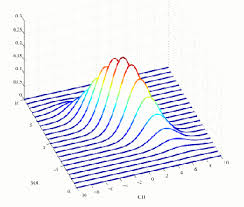
\includegraphics[width=0.7\linewidth]{BivariateNormal1}
	\end{figure}
Bivariate describes the case of two variables.
\end{frame}
%=================================================================================================% 
\begin{frame}[fragile]
\frametitle{Bivariate Normality}

\begin{figure}[h!]
\centering
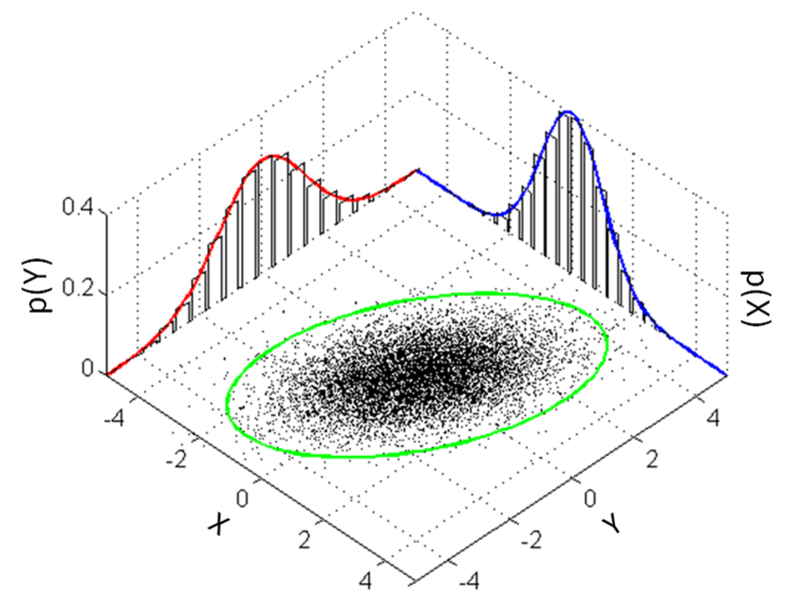
\includegraphics[width=0.95\linewidth]{./images/793px-MultivariateNormal}
\end{figure}
	
\end{frame}


%=================================================================================================% 
\begin{frame}[fragile]
\frametitle{Testing for Normality}
	{
	\noindent\textbf{Hypothesis Tests for Univariate Data}
	
	\bigskip		\large
		\textbf{Graphical Methods}
		\begin{itemize}
			\item Histograms (with Kerney Density Estimation Line)
			\item Normal Probability Plots
		\end{itemize}
		\bigskip		\large
		\textbf{Formal Hypothesis Tests}
			\begin{itemize}
				\item Shapiro-Wilk Test (inbuilt with \texttt{R})
				\item Anderson-Darling Test (nortest package)
				\item D'Agostino Test (MSQC package)
			\end{itemize}
	}
\end{frame}

%=================================================================================================% 
\begin{frame}[fragile]
	\frametitle{Testing for Normality}

	
	\noindent\textbf{Hypothesis Tests for Multivariate Data}
	\begin{itemize}
		\item Mardia Test (MSQC package)
		\item Henze and Zirkler (MSQC package)
		\item Royston Test (MSQC package)
	\end{itemize}
\end{frame}
%=================================================================================================% 
\begin{frame}[fragile]
	\frametitle{Testing for Normality}
	
	\textbf{The bimetal data set (MSQC package)}
	{\large
		\begin{itemize}
			\item Bimetal thermostat has innumerable practical uses. These types of thermostats hold
			a bimetallic strip composed by two strips of different metals that convert the
			changing of temperature in mechanical displacement due to the difference in
			thermal expansion.
			\item Certain type of strip composed of brass and steel is analyzed in a quality
			laboratory by testing the deflection, curvature, resistivity, and hardness in low
			and high expansion sides.
		\end{itemize}
	}
	\end{frame}

%=================================================================================================% 
	\begin{frame}[fragile]
		\frametitle{Testing for Normality}
\large
\begin{verbatim}
			> tail(bimetal1)
			deflection curvature resistivity Hardness low side Hardness high side
			[23,]      20.76     39.98       14.98             22.29             26.03
			[24,]      21.00     40.11       15.17             22.04             25.99
			[25,]      20.57     39.73       14.35             22.02             25.80
			[26,]      20.78     39.83       15.27             21.60             25.89
			[27,]      20.96     40.03       15.26             21.98             25.94
			[28,]      21.14     39.93       14.98             21.84             25.98
\end{verbatim}
\end{frame}

%=================================================================================================% 
\begin{frame}[fragile]
\frametitle{Testing for Normality}
\begin{figure}[h!]
\centering
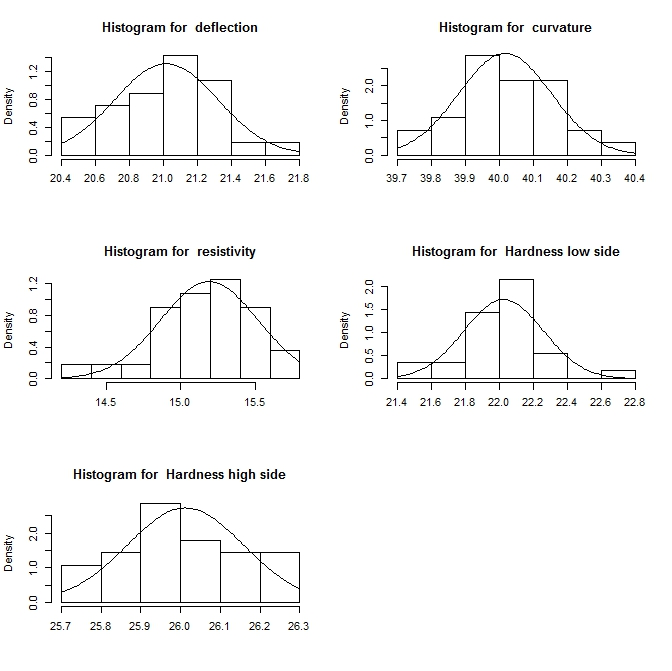
\includegraphics[width=0.8\linewidth]{images/MSQC-bimetal1hist}
\end{figure}
	\end{frame}
	
%\end{document}
%=================================================================================================% 
\begin{frame}[fragile]
\frametitle{Testing for Normality}
\begin{figure}[h!]
\centering
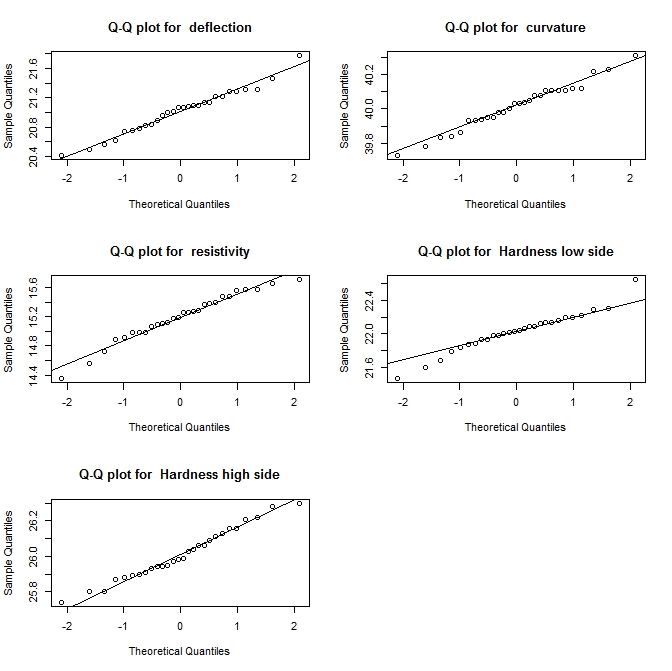
\includegraphics[width=0.8\linewidth]{images/MSQC-bimetal1qq}
\end{figure}
\end{frame}
%\end{document}
%=================================================================================================% 
\begin{frame}
	\frametitle{Skewness and Kurtosis}
\begin{itemize}
\item Skewness is a measure of symmetry, or more precisely, the lack of symmetry. A distribution, or data set, is symmetric if it looks the same to the left and right of the center point.

\item Kurtosis is a measure of whether the data are peaked or flat relative to a normal distribution. That is, data sets with high kurtosis tend to have a distinct peak near the mean, decline rather rapidly, and have heavy tails. Data sets with low kurtosis tend to have a flat top near the mean rather than a sharp peak.
\end{itemize}
\end{frame}
%============================================================ %

\begin{frame}
\frametitle{Skewness and Kurtosis}
\large
\begin{itemize}
\item	The normal distribution is a symmetric distribution with well-behaved tails. 
\item Theoretically a Normal Distibuted Random Variable will have a skewness of 0.00. 
\item	Also The kurtosis of 2.96 is near the expected value of 3.
\end{itemize}

\end{frame}
%============================================================ %
\begin{frame}
\frametitle{Skewness}
	\begin{figure}
\centering
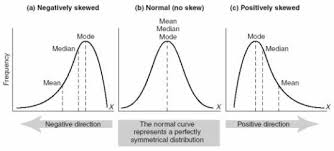
\includegraphics[width=0.85\linewidth]{images/skewness2}
\end{figure}
\begin{itemize}
\item Negatively Skewed  - Skewness is negative number
\item Symmetric  - Skewness is zero
\item Positively Skewed - Skewness is positive number
\end{itemize}
\end{frame}
%============================================================= %
\begin{frame}
	\begin{figure}
\centering
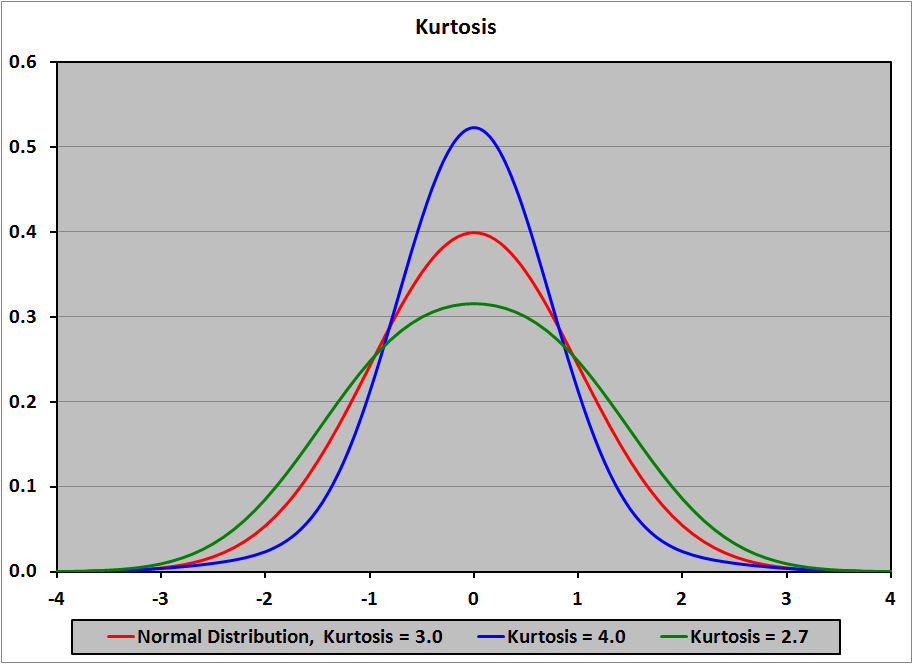
\includegraphics[width=0.7\linewidth]{images/Kurtosis-Chart}
\caption{}
\label{fig:Kurtosis-Chart}
\end{figure}

\end{frame}
%=================================================================================================% 
\begin{frame}
\frametitle{D'Agostino Test}
\Large
\begin{itemize}
\item D’Agostino’s $K^2$ test, named for Ralph D'Agostino, is a goodness-of-fit measure of departure from normality, that is the test aims to establish whether or not the given sample comes from a normally distributed population. 
\item The test is based on transformations of the \textbf{sample kurtosis} and \textbf{skewness}, and has power only against the alternatives that the distribution is skewed and/or kurtic.
\end{itemize}
\end{frame}
%=================================================================================================% 
\begin{frame}[fragile]
\frametitle{Testing for Normality}
\noindent	\textbf{D'Agostino Test (MSQC Package)}
			\begin{itemize}
				\item Using the bimetal1 data set in MSQC package
\item Run the procedure on the first variable only.
			\end{itemize}
			\begin{framed}
				\begin{verbatim}
	 library(MSQC)
	 DAGOSTINO(bimetal1[,1])
				
			\end{verbatim}
			\end{framed}
			Output on next two slides
\end{frame}
%\end{document}
%=================================================================================================% 
				\begin{frame}[fragile]
				\frametitle{Testing for Normality}
				\begin{framed}
				\begin{verbatim}
				D'Agostino Test
				
				Skewness
				Skewness coefficient: 0.0831225 
				Statistics: 0.2117358 
				p-value: 0.8323131 
				
				Kurtosis
				The kurtosis coefficient: 3.0422 
				Statistics: 0.591983 
				p-value: 0.553862 
						\end{verbatim}
					\end{framed}
				\end{frame}
				%=================================================================================================% 
				\begin{frame}[fragile]
					\frametitle{Testing for Normality}
					\begin{framed}
						\begin{verbatim}
						....
				Omnibus Test
				Chi-squared: 0.3952759 
				Degree of freedom: 2
				p-value: 0.8206669 
				\end{verbatim}
			\end{framed}
				\end{frame}
				%=================================================================================================% 
				\begin{frame}[fragile]
					\begin{itemize}
						\item Mardia Test is a multivariate test based in multivariate Skewness and Multivariate Kurtosis. 
						\item Those topics are outside the scope of the course.
						
					\end{itemize}
				\end{frame}
%=================================================================================================% 
\begin{frame}[fragile]
			\frametitle{Testing for Normality}
			\textbf{Some Multivariate (MSQC Package)}
			\begin{framed}
				\begin{verbatim}
				> MardiaTest(bimetal1)
				$skewness
				[1] 6.982112
				
				$p.value
				[1] 0.585327
				
				$kurtosis
				[1] 33.77373
				
				$p.value
				[1] 0.3490892
						\end{verbatim}
					\end{framed}
				\end{frame}
				%=================================================================================================% 
				\begin{frame}[fragile]
				\frametitle{Testing for Normality}
				\begin{framed}
					\begin{verbatim}
				>
				> HZ.test(bimetal1)
				[1] 0.6068650 0.7709586
				> 
						\end{verbatim}
					\end{framed}
				\end{frame}
				%=================================================================================================% 
				\begin{frame}[fragile]
				\frametitle{Testing for Normality}
					\begin{framed}
						\begin{verbatim}
				> Royston.test(bimetal1)
				test.statistic        p.value 
				1.1814742      0.9364221 
				\end{verbatim}
			\end{framed}
			
		\end{frame}
		%=================================================================================================% 
		\begin{frame}[fragile]
			\frametitle{Testing for Normality}
			
			\textbf{Box Cox Transformation}
			\begin{itemize}
				\item The Box-Cox transforms non-normally distributed data to a set of data that has approximately normal distribution. 
			\end{itemize}
		\end{frame}
		
	\end{document}